%!TEX TS-program = xelatex
%!TEX encoding = UTF-8 Unicode

\documentclass[galley]{jtlu-article-2col}
\usepackage{tabu}
\renewcommand\query[1]{\relax}

\graphicspath{{../Graphics/},{../../../../jtlugraphics/}}

%% ===== BEGIN ARTICLE DATA BLOCK - FILL IN THIS STUFF ==== %%
%% ===== JTLU publication and copyright info (required) === %%
\jtluissue{1}
\jtluvolume{7}
\jtluyear{2014}
\jtlurights{Robin Lovelace}
\jtluid{nnn}
\setcounter{page}{1}

%% ===== ARTICLE TITLE (required), subtitle (optional) ==== %%
\title{Combining origin-destination and spatial network approaches to estimate walking and cycling potential}
%\subtitle{Subtitle in sentence case}

%% ===== SHORT TITLE (required for page headers) ========== %%
\shorttitle{}

%% ===== AUTHOR INFORMATION (required) ==================== %%
%% Name, affiliation/institution, and email/contact for each
%% Add as many as necessary, separated by "\and":

\author{{\semibfsf Robin Lovelace  } \\University of Leeds  \thanks{r.lovelace@ leeds.ac.uk}
  \and {\bfseries Crispin Cooper} \\University of Cardiff
  % \and {\bfseries } \\
  % \and {\bfseries } \\
}% End authors

%% ===== END ARTICLE DATA BLOCK =========================== %%

\date{} % SET DATE TO NOTHING; NO DATE ON PAPERS

\hypersetup{%
			pdftitle={Combining origin-destination and spatial network approaches to estimate walking and cycling potential},
			pdfauthor={Robin Lovelace},
			pdfproducer={The Journal of Transport and Land Use vol. 7 no. 1 }
			pdfstartpage=1,
			colorlinks=true,
			linkcolor=NavyBlue,
			citecolor=PineGreen,
			urlcolor=BrickRed
} % END HYPERSETUP


% For figures and more when knitting from .Rmd:
% https://stackoverflow.com/questions/41052687/
\providecommand{\tightlist}{%
  \setlength{\itemsep}{0pt}\setlength{\parskip}{0pt}}
\usepackage{longtable,booktabs,array}
\newlength{\cslhangindent}
\setlength{\cslhangindent}{1.5em}
\newlength{\csllabelwidth}
\setlength{\csllabelwidth}{3em}
\newenvironment{CSLReferences}[2] % #1 hanging-ident, #2 entry spacing
 {% don't indent paragraphs
  \setlength{\parindent}{0pt}
  % turn on hanging indent if param 1 is 1
  \ifodd #1 \everypar{\setlength{\hangindent}{\cslhangindent}}\ignorespaces\fi
  % set entry spacing
  \ifnum #2 > 0
  \setlength{\parskip}{#2\baselineskip}
  \fi
 }%
 {}
\usepackage{calc}
\newcommand{\CSLBlock}[1]{#1\hfill\break}
\newcommand{\CSLLeftMargin}[1]{\parbox[t]{\csllabelwidth}{#1}}
\newcommand{\CSLRightInline}[1]{\parbox[t]{\linewidth - \csllabelwidth}{#1}\break}
\newcommand{\CSLIndent}[1]{\hspace{\cslhangindent}#1}

% Custom add-ons
\usepackage[no-math]{fontspec}


\begin{document}
\twocolumn[
\begin{@twocolumnfalse}
\maketitle

\begin{abstract}
Add your article abstract here,
test test test.
lots and lots
and lots and lots
of text\ldots\ldots\ldots\ldots\ldots\ldots\ldots\ldots\ldots\ldots\ldots\ldots.
\end{abstract}

\begin{keywords}
  Keyword 1; keyword 2;
\end{keywords}
\end{@twocolumnfalse}
]
\saythanks

\hypertarget{introduction}{%
\section{Introduction}\label{introduction}}

There has been much research on mode shift since the origins of applied transport planning and modelling in the 1950s (Boyce and Williams 2015; Aguil'era and Gr'ebert 2014). Within this broad field of research, uptake of `active modes' (walking and cycling) has become a recent focus (Götschi et al. 2017). A range of methods have been used to understand and model walking and cycling levels, with `getting people cycling' being the topic of numerous papers during the 2010 (e.g. Beecham, Wood, and Bowerman 2012; Gris'e and El-Geneidy 2018; Larsen, Patterson, and El-Geneidy 2013; Raffler, Brezina, and Emberger 2019; Zhang, Magalhaes, and Wang 2014).

Within the wide range of approaches used to model cycling uptake, two broad approaches have been particularly prominent in the literature. The \emph{origin-destination approach} relies on estimates of current travel behaviour, represented in origin-destination datasets reporting the number of trips, e.g.~by mode of travel to work on a typical working day between residential zone origins and workplace destinations. This approach was used in the Propensity to Cycle Tool (PCT), which was originally developed to support strategic cycle network planning based on commuter data for England (Lovelace et al. 2017). The `PCT approach,' which is a particular implementation of the `origin-destination' approach that models cycling uptake in terms of `distance-hilliness decay' functions (which can include other explanatory variables such as traffic levels) has subsequently been adapted to explore cycling potential in other contexts, including cycling uptake in US cities with low cycling levels (Ahmad et al. 2020) and the potential for mode shift to cycling for the `school commute' in across all state schools in England, with publicly available visualisations down to the street level (Goodman et al. 2019).

The aim of this paper is to demonstrate the relative merits of the `origin-destination approach' implemented in the PCT and the `spatial network' approach implemented in the open source sDNA software (Chan and Cooper 2019).
We do so using reproducible methods and open access input data to encourage others to employ the techniques in other areas to support evidence-based interventions to enable cycling uptake and as a basis for future research and development.

\hypertarget{study-area-and-input-data}{%
\section{Study area and input data}\label{study-area-and-input-data}}

The case study area is the local authority district of Monmouthshire, in rural South Wales (Figure \ref{fig:case}). The research took place in the context of the Welsh Active Travel Act (Welsh Government 2020).

\begin{figure}
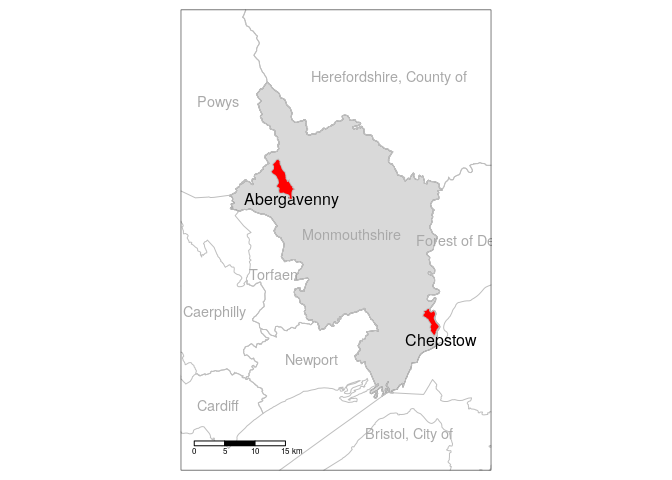
\includegraphics[width=9.33in]{README_files/figure-gfm/unnamed-chunk-4-1} \caption{Case study area, with the parishes of Chepstow and Abergavenny highlighted in red.}\label{fig:case}
\end{figure}

The main destinations of interest were schools and leisure centres.
These can be obtained from OpenStreetMap with the tags (key-value pairs) \texttt{amenity=school} and \texttt{leisure=sports\_centre}.

Other than destinations of interest, the other key input was the boundary of the region responsible for the transport system in the local area.
We tested two approaches to define the `area of interest' defining the area within which routes were calculated: a simple buffer and a three-stage buffering process, as illustrated in Figure \ref{fig:buffers}.
The simple buffer approach involved creating polygon with borders a fixed distance (5 km in the first instance) around the destination (in this case the parishes of Chepstown and Abergavenny).
Model run times (and visualisation load times in interactive maps) depend on the amount of data served, creating an incentive reduce the size of the input data, and from a policy perspective, it makes sense to focus on the area over which local planners have control (and budget).
In this context, the three-stage process was developed as follows:

\begin{enumerate}
\def\labelenumi{\arabic{enumi}.}
\tightlist
\item
  Create a buffer around the zone of interest with a threshold distance (set to 5 km)
\item
  Create a separate buffer around the region of interest to allow for some (more limited) inter-regional flow (set to 2 km)
\item
  Calculate the intersection between the two buffers outlined in the previous stages
\end{enumerate}

\begin{figure}
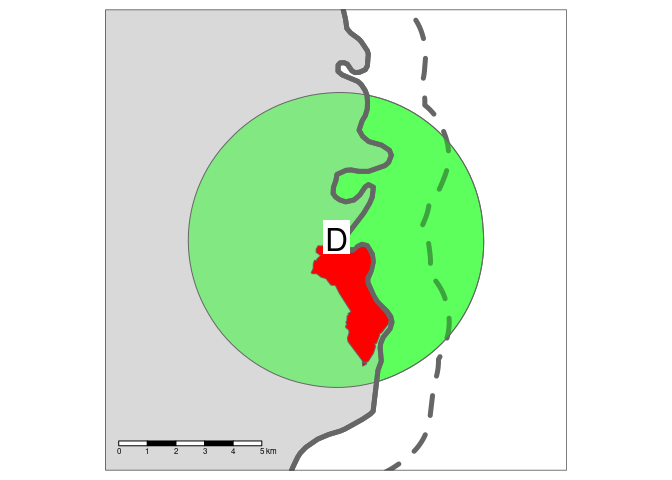
\includegraphics[width=0.49\linewidth]{README_files/figure-latex/buffers-1} 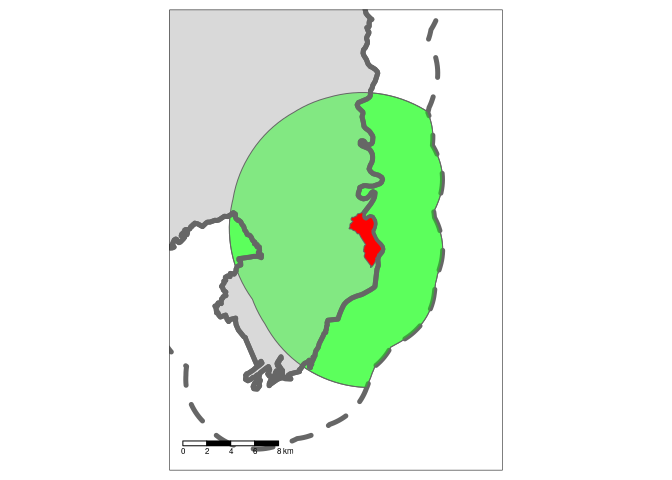
\includegraphics[width=0.49\linewidth]{README_files/figure-latex/buffers-2} \caption{Illustration of the simple buffer and three stage buffering approaches to identify areas of interest within which travel to destinations in the zones could take place. The D represents the desination of interest.}\label{fig:buffers}
\end{figure}

A key input is origin-destination (OD) data.
OD data can be obtained from a number of sources, the most reliable being a list of geocoded addresses or postcodes associated with people who visit each destination regularly.
In cases where OD datasets derived from from surveys or official/commercial records are missing, they can be simulated using a range of techniques.
For the purposes of this paper, to enable full reproducibility, we simulate origins by sampling from buildings in the study area, as illustrated below.

\begin{figure}
\centering
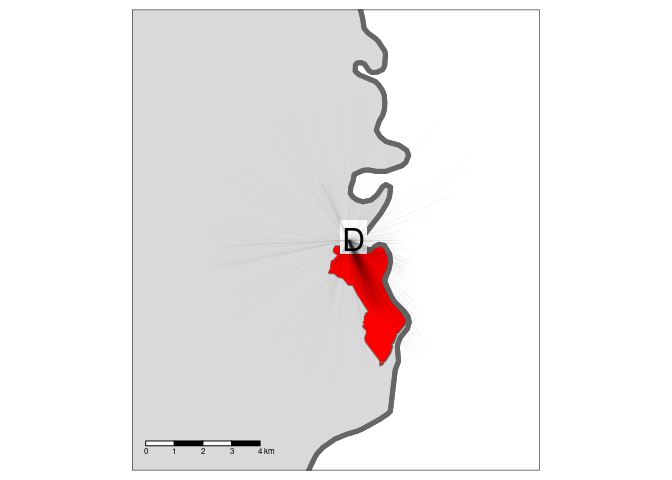
\includegraphics{README_files/figure-latex/unnamed-chunk-11-1.pdf}
\caption{\label{fig:unnamed-chunk-11}Origin-destination data, represented as `desire lines' emanating from residential origins with the destination fixed to the destination.}
\end{figure}

The other key input, for spatial network analysis, is route network data.
This can be obtained from OpenStreetMap, which has global coverage (although quality varies).
The OSM data

\hypertarget{origin-destination-analysis}{%
\section{Origin-destination analysis}\label{origin-destination-analysis}}

Describe a generalised version of the `PCT approach' with recent modifications, improvements and areas for improvement (RL)

\hypertarget{origin-destination-data-processing}{%
\subsection{Origin-destination data processing}\label{origin-destination-data-processing}}

Talk about data availability, possibility of modelling OD data with SIMs and od package (RL)

\hypertarget{routing-od-data}{%
\subsection{Routing: OD data}\label{routing-od-data}}

Different routing options (RL)

\hypertarget{estimating-cycling-uptake}{%
\subsection{Estimating cycling uptake}\label{estimating-cycling-uptake}}

Go Dutch and other options (RL)

\hypertarget{spatial-network-analysis}{%
\section{Spatial network analysis}\label{spatial-network-analysis}}

Explanation of the method and reproducible example (CC)

\hypertarget{spatial-network-processing}{%
\subsection{Spatial network processing}\label{spatial-network-processing}}

\hypertarget{network-modelling}{%
\subsection{Network modelling}\label{network-modelling}}

\hypertarget{scenario-analysis}{%
\subsection{Scenario analysis}\label{scenario-analysis}}

How the walking/cycling scenarios were implemented with sDNA (CC)

\hypertarget{integrated-od-and-sna-network-analysis}{%
\section{Integrated OD and SNA network analysis}\label{integrated-od-and-sna-network-analysis}}

RL + CC

\hypertarget{road-network-visualisation}{%
\subsection{Road network visualisation}\label{road-network-visualisation}}

\hypertarget{findings}{%
\section{Findings}\label{findings}}

RL + CC

\hypertarget{conclusions}{%
\section{Conclusions}\label{conclusions}}

RL + CC

\hypertarget{references}{%
\section*{References}\label{references}}
\addcontentsline{toc}{section}{References}

\hypertarget{refs}{}
\begin{CSLReferences}{1}{0}
\leavevmode\hypertarget{ref-aguilera_passenger_2014}{}%
Aguil'era, Anne, and Jean Gr'ebert. 2014. {``Passenger Transport Mode Share in Cities: Exploration of Actual and Future Trends with a Worldwide Survey.''} \emph{International Journal of Automotive Technology and Management} 14 (3-4): 203--16. \url{https://doi.org/10.1504/IJATM.2014.065290}.

\leavevmode\hypertarget{ref-ahmad_comparison_2020}{}%
Ahmad, Sohail, Anna Goodman, Felix Creutzig, James Woodcock, and Marko Tainio. 2020. {``A Comparison of the Health and Environmental Impacts of Increasing Urban Density Against Increasing Propensity to Walk and Cycle in {Nashville}, {USA}.''} \emph{Cities \& Health} 4 (1): 55--65. \url{https://doi.org/10.1080/23748834.2019.1659667}.

\leavevmode\hypertarget{ref-beecham_visual_2012}{}%
Beecham, Roger, Jo Wood, and Audrey Bowerman. 2012. {``A Visual Analytics Approach to Understanding Cycling Behaviour.''} In \emph{2012 {IEEE Conference} on {Visual Analytics Science} and {Technology} ({VAST})}, 207--8. {IEEE}.

\leavevmode\hypertarget{ref-boyce_forecasting_2015}{}%
Boyce, David E., and Huw C. W. L. Williams. 2015. \emph{Forecasting {Urban Travel}: {Past}, {Present} and {Future}}. {Edward Elgar Publishing}.

\leavevmode\hypertarget{ref-chan_using_2019}{}%
Chan, Eric Yin Cheung, and Crispin HV Cooper. 2019. {``Using Road Class as a Replacement for Predicted Motorized Traffic Flow in Spatial Network Models of Cycling.''} \emph{Scientific Reports} 9 (1): 1--12.

\leavevmode\hypertarget{ref-goodman_scenarios_2019}{}%
Goodman, Anna, Ilan Fridman Rojas, James Woodcock, Rachel Aldred, Nikolai Berkoff, Malcolm Morgan, Ali Abbas, and Robin Lovelace. 2019. {``Scenarios of Cycling to School in {England}, and Associated Health and Carbon Impacts: {Application} of the {`{Propensity} to {Cycle Tool}'}.''} \emph{Journal of Transport \& Health} 12 (March): 263--78. \url{https://doi.org/10.1016/j.jth.2019.01.008}.

\leavevmode\hypertarget{ref-gotschi_comprehensive_2017}{}%
Götschi, Thomas, Audrey de Nazelle, Christian Brand, Regine Gerike, and Regine Gerike. 2017. {``Towards a {Comprehensive Conceptual Framework} of {Active Travel Behavior}: A {Review} and {Synthesis} of {Published Frameworks}.''} \emph{Current Environmental Health Reports} 4 (3): 286--95. \url{https://doi.org/10.1007/s40572-017-0149-9}.

\leavevmode\hypertarget{ref-grise_if_2018}{}%
Gris'e, Emily, and Ahmed El-Geneidy. 2018. {``If We Build It, Who Will Benefit? {A} Multi-Criteria Approach for the Prioritization of New Bicycle Lanes in {Quebec City}, {Canada}.''} \emph{Journal of Transport and Land Use} 11 (1). \url{https://doi.org/10.5198/jtlu.2018.1115}.

\leavevmode\hypertarget{ref-larsen_build_2013}{}%
Larsen, Jacob, Zachary Patterson, and Ahmed El-Geneidy. 2013. {``Build It. {But} Where? {The} Use of Geographic Information Systems in Identifying Locations for New Cycling Infrastructure.''} \emph{International Journal of Sustainable Transportation} 7 (4): 299--317.

\leavevmode\hypertarget{ref-lovelace_propensity_2017}{}%
Lovelace, Robin, Anna Goodman, Rachel Aldred, Nikolai Berkoff, Ali Abbas, and James Woodcock. 2017. {``The {Propensity} to {Cycle Tool}: {An} Open Source Online System for Sustainable Transport Planning.''} \emph{Journal of Transport and Land Use} 10 (1). \url{https://doi.org/10.5198/jtlu.2016.862}.

\leavevmode\hypertarget{ref-raffler_cycling_2019}{}%
Raffler, Clemens, Tadej Brezina, and Günter Emberger. 2019. {``Cycling Investment Expedience: {Energy} Expenditure Based {Cost}-{Path Analysis} of National Census Bicycle Commuting Data.''} \emph{Transportation Research Part A: Policy and Practice} 121 (March): 360--73. \url{https://doi.org/10.1016/j.tra.2019.01.019}.

\leavevmode\hypertarget{ref-welshgovernment_active_2020}{}%
Welsh Government. 2020. {``Active {Travel Guidance}.''} {Welsh Government}.

\leavevmode\hypertarget{ref-zhang_prioritizing_2014}{}%
Zhang, Dapeng, David Jose Ahouagi Vaz Magalhaes, and Xiaokun (Cara) Wang. 2014. {``Prioritizing Bicycle Paths in {Belo Horizonte City}, {Brazil}: {Analysis} Based on User Preferences and Willingness Considering Individual Heterogeneity.''} \emph{Transportation Research Part A: Policy and Practice} 67: 268--78. \url{https://doi.org/10.1016/j.tra.2014.07.010}.

\end{CSLReferences}

% \section{Introduction}
%
%
%
%
%
% \section{Section name}
% \label{sec:section-name}
%
%
%
% \subsection{Subsection heading}


%%%%%%%%%%
% \begin{figure*}[htbp]
%   \centering
%   \includegraphics{fig1}
%   \caption{Caption ...  }
%   \label{fig:1}
% \end{figure*}



\bibliographystyle{jtlu}
\bibliography{../Bib/filename}

\end{document}
